\chapter{Getting started} 

\section{Basic Settings}
\begin{itemize}
  \item \textbf{system:} Ubuntu 16.04 LTS
  \item \textbf{ROS:} kinetic-1.12.7
  \item \textbf{morse:} morse-1.3-Stable
  \item \textbf{blender} blender-2.76
  \item some useful links that may help you:
  \begin{enumerate}
  	\item This project can be found in:
	  	\begin{itemize}
			\item \textcolor{red}{https://gitlab.tubit.tu-berlin.de/aac-hrc/emphatic-hrc-boxing}
		\end{itemize}
  	\item morse and ROS:
	  	\begin{itemize}
  			\item \textcolor{red}{http://www.openrobots.org/morse/doc/stable/morse.html}
  			\item \textcolor{red}{http://wiki.ros.org/kinetic/Installation/Ubuntu}
  			\item \textcolor{red}{https://www.openrobots.org/morse/doc/latest/user/beginner\_t\\utorials/ros\_tutorial.html}
  			\item \textcolor{red}{http://www.openrobots.org/morse/doc/1.3/user/beginner\_t\\utorials/hri\_tutorial.html}
		\end{itemize}
  	\item MDP/POMDP:
	  	\begin{itemize}
  			\item \textcolor{red}{http://pomdp.org/}
  			\item \textcolor{red}{http://bigbird.comp.nus.edu.sg/pmwiki/farm/appl/index.php?n\\=Main.Download}
  			\item \textcolor{red}{http://bigbird.comp.nus.edu.sg/pmwiki/farm/appl/uploads/Ma\\in/README-0.96.txt}
		\end{itemize}
  \end{enumerate}
\end{itemize}

\section{Compile}

\subsection{MDP}
navigate to code/despot\_MDP:\\
\colorbox{gray}{\begin{minipage}{\linewidth} mkdir build \end{minipage}}\\
\colorbox{gray}{\begin{minipage}{\linewidth} cd build \end{minipage}}\\
\colorbox{gray}{\begin{minipage}{\linewidth} cmake .. \end{minipage}}\\
\colorbox{gray}{\begin{minipage}{\linewidth} make \end{minipage}}\\

\subsection{POMDP}
navigate to code/despot\_POMDP:\\
\colorbox{gray}{\begin{minipage}{\linewidth} mkdir build \end{minipage}}\\
\colorbox{gray}{\begin{minipage}{\linewidth} cd build \end{minipage}}\\
\colorbox{gray}{\begin{minipage}{\linewidth} cmake .. \end{minipage}}\\
\colorbox{gray}{\begin{minipage}{\linewidth} make \end{minipage}}\\

\subsection{ROS}
navigate to code/ros\_ws:\\
\colorbox{gray}{\begin{minipage}{\linewidth} catkin\_make \end{minipage}}\\

\subsection{morse}
The morse open source codes are not well developed and they lack a lot of functionalities that we need in this project. We complement the source codes of morse with our own codes. In order to successfully run the project, you need to add or replace some of the source codes by following the instructions below. To make sure that you don't lose original source codes, we recommend you to make a copy before replacing them.
\begin{enumerate}\setlength{\itemsep}{0.05cm}
\item navigate to code/hrc\_morse/src:
	\begin{enumerate}\setlength{\itemsep}{0.02cm}
	\item replace human.py:\\
	\colorbox{gray}{\begin{minipage}{\linewidth} sudo cp human.py /opt/lib/python3/dist-packages/morse/robots/ \end{minipage}}
	\item replace pr2.py: \\
	\colorbox{gray}{\begin{minipage}{\linewidth} sudo cp pr2.py /opt/lib/python3/dist-packages/morse/robots/ \end{minipage}}
	\item replace main.py: \\
	\colorbox{gray}{\begin{minipage}{\linewidth} sudo cp main.py /opt/lib/python3/dist-packages/morse/blender/ \end{minipage}}
	\end{enumerate}
\item navigate to code/hrc\_morse/data:
	\begin{enumerate}\setlength{\itemsep}{0.02cm}
	\item replace human.blend: \\
	\colorbox{gray}{\begin{minipage}{\linewidth} sudo cp human.blend /opt/share/morse/data/robots/  \end{minipage}}
	\item replace pr2.blend: \\
	\colorbox{gray}{\begin{minipage}{\linewidth} sudo cp pr2.blend /opt/share/morse/data/robots/  \end{minipage}}
	\item add a conveyor belt: \\
	\colorbox{gray}{\begin{minipage}{\linewidth} sudo cp conveyor.blend /opt/share/morse/data/environments/  \end{minipage}}
	\end{enumerate}
\item Now you can create a morse workspace(named as "hrc") and put our morse script file into it:\\
\colorbox{gray}{\begin{minipage}{\linewidth} morse create YOUR\_MORSE\_PATH/hrc \end{minipage}}
navigate to code/hrc\_morse:\\
\colorbox{gray}{\begin{minipage}{\linewidth} cp builder\_script.py YOUR\_MORSE\_PATH/hrc/ \end{minipage}}
\end{enumerate}

\section{Run an Example}
In this section, we show how to run a complete HRC example scenario. All the tools, including morse, blender, ROS, MDP and POMDP, are manipulated via commands from ternimal.
\begin{enumerate}\setlength{\itemsep}{0.05cm}
	\item initialize ROS:\\
	\colorbox{gray}{\begin{minipage}{\linewidth} roscore \end{minipage}}
	\item run morse scenario:\\
	in a new terminal, navigate to YOUR\_MORSE\_PATH/:\\
	\colorbox{gray}{\begin{minipage}{\linewidth} morse run builder\_script.py \end{minipage}}
	\item run ROS nodes:\\
	in a new ternimal, navigate to code/ros\_ws:\\
	\colorbox{gray}{\begin{minipage}{\linewidth} source devel/setup.bash \end{minipage}}
	\colorbox{gray}{\begin{minipage}{\linewidth} roslaunch ros\_hrc hrc.launch \end{minipage}}
	\item If everything runs successfully, you will see besides current three terminal windows(see Fig \ref{fig:roscorerun}, Fig \ref{fig:morserun}, Fig \ref{fig:ROSnoderun}), there are two new terminal windows poping up: one window runs MDP(from despot\_MDP, see Fig \ref{fig:MDPrun}) and the other runs POMDP(from despot\_POMDP, see Fig \ref{fig:POMDPrun}). Fig \ref{fig:morsescenario} shows the simulation scenario.

\begin{minipage}{0.3\textwidth}
\centering
	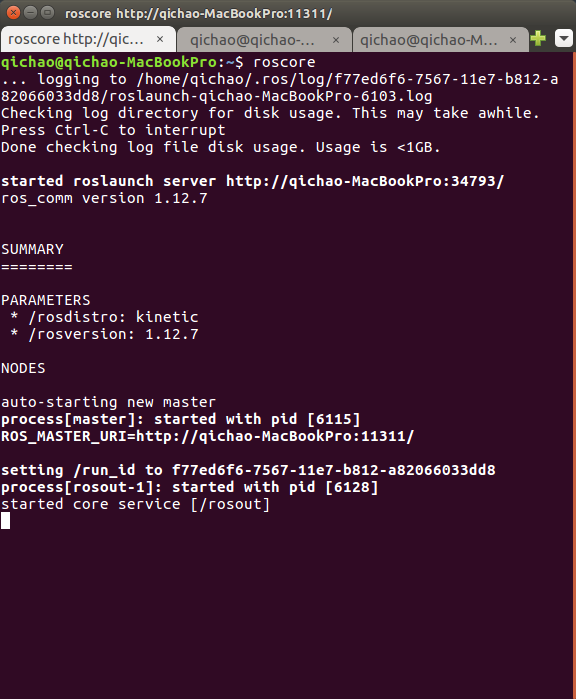
\includegraphics[width=4cm]{Pictures/run/roscorerun.png}
	\captionof{figure}{roscore}
	\label{fig:roscorerun}
\end{minipage}
\quad
\begin{minipage}{0.3\textwidth}
\centering
	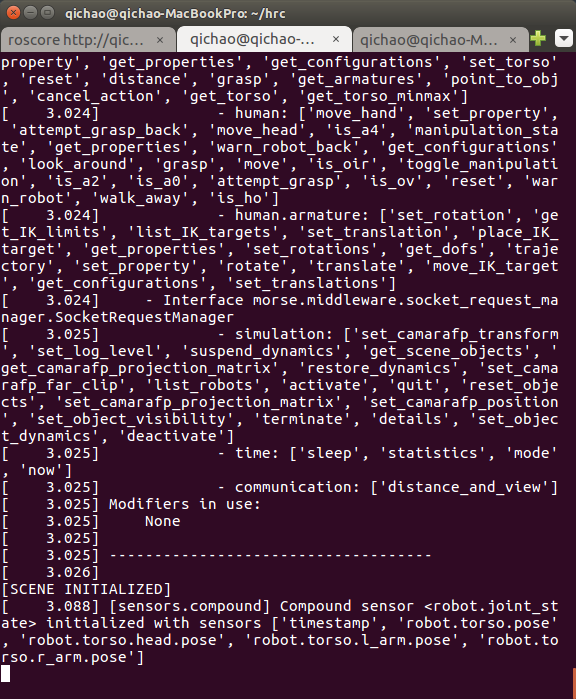
\includegraphics[width=4cm]{Pictures/run/morserun.png}
	\captionof{figure}{morse}
	\label{fig:morserun}
\end{minipage}
\quad
\begin{minipage}{0.3\textwidth}
\centering
	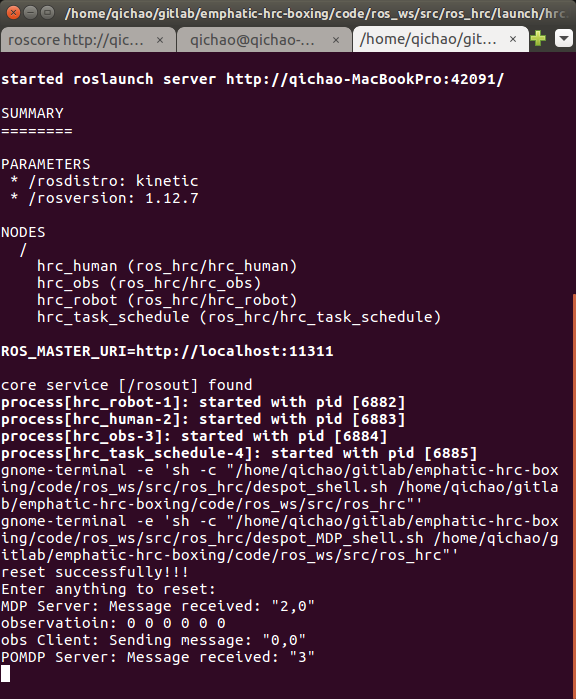
\includegraphics[width=4cm]{Pictures/run/ROSnoderun.png}
	\captionof{figure}{ROS}
	\label{fig:ROSnoderun}
\end{minipage}

\begin{minipage}{0.3\textwidth}
\centering
	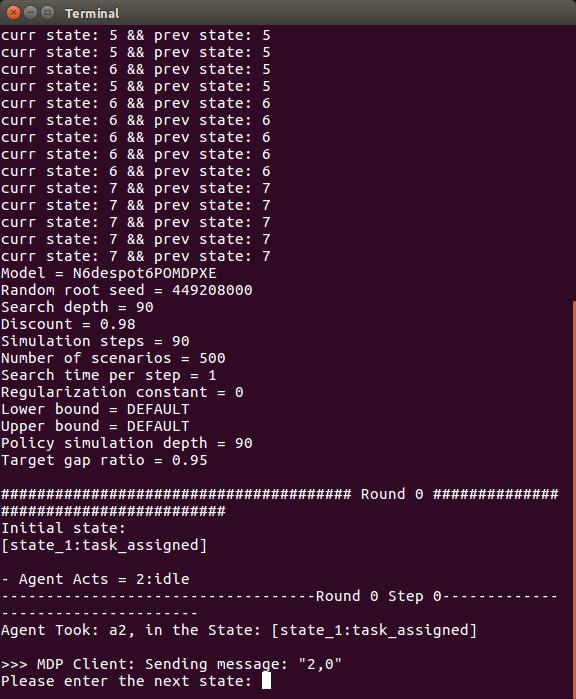
\includegraphics[width=4cm]{Pictures/run/MDPrun.png}
	\captionof{figure}{MDP}
	\label{fig:MDPrun}
\end{minipage}
\quad
\begin{minipage}{0.3\textwidth}
\centering
	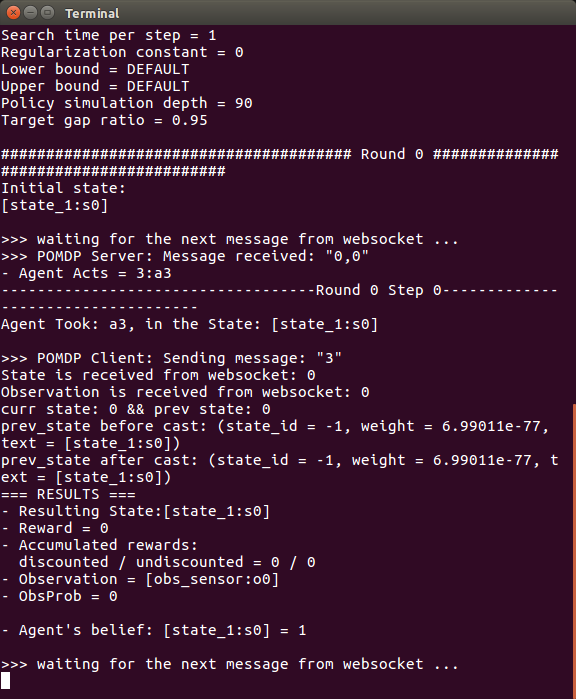
\includegraphics[width=4cm]{Pictures/run/POMDPrun.png}
	\captionof{figure}{POMDP}
	\label{fig:POMDPrun}
\end{minipage}

	\item You can control the behavious of human only by inputing the next state of MDP from the MDP terminal(Fig \ref{fig:MDPrun}). When you input a proper integer in the MDP terminal(there are 8 states: 0 is initial state; you can input 1-7), ROS terminal(Fig \ref{fig:ROSnoderun}) will output the current human action, human observation, robot observation, human state, robot state, as well as robot action, where the robot action is calculated in POMDP and transfered to ROS via webSocket. As a result, this action is executed in morse.
	\item At any time, you can press "Enter" in the ROS terminal(Fig \ref{fig:ROSnoderun}) to reset the whole scenario. Before reset, you should manually close the MDP and POMDP terminal windows.
	
\begin{minipage}{0.8\textwidth}
\centering
	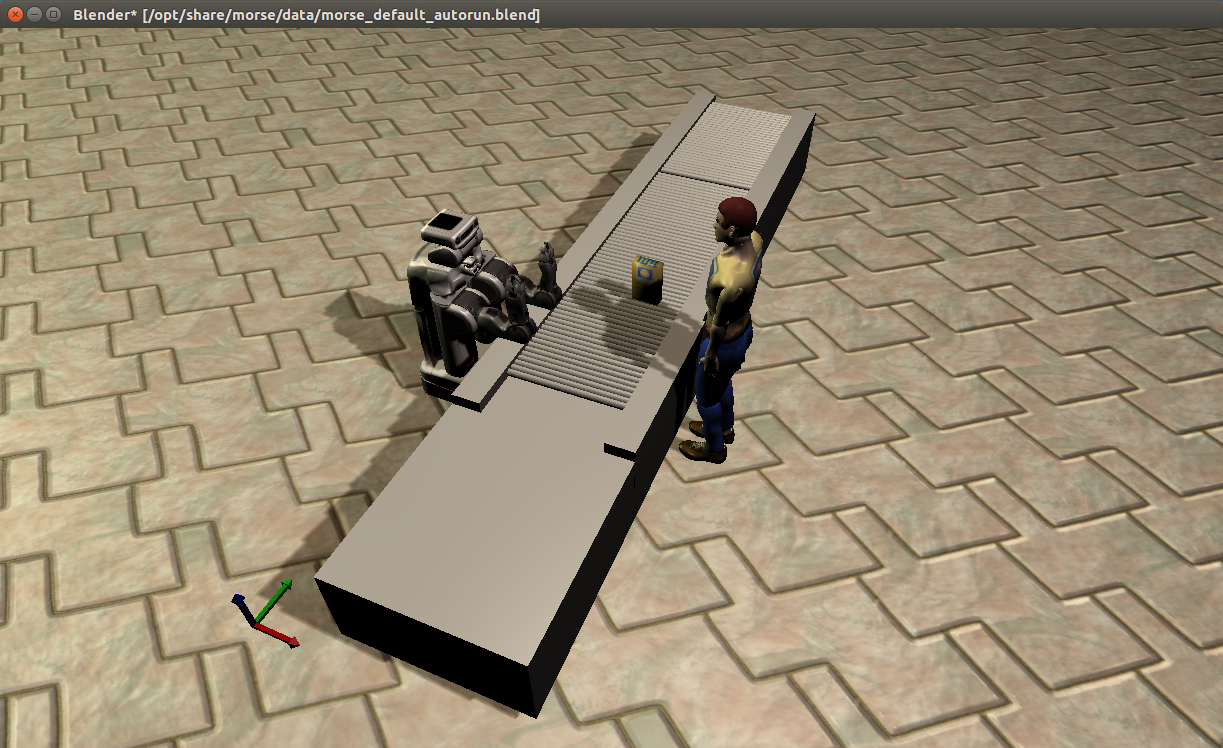
\includegraphics[width=12cm]{Pictures/run/morsescenario.png}
	\captionof{figure}{morse scenario}
	\label{fig:morsescenario}
\end{minipage}

\end{enumerate}

\chapter{Theoretical Explanation} 

\section{Architecture and Communication graph}
Fig \ref{fig:architecture} shows the genaral architure of the project. Fig \ref{fig:graph} shows how we use webSocket and ROS service to transfer information and communicate between different components(morse, ROS, MDP and POMDP).

\begin{minipage}{0.8\textwidth}
\centering
	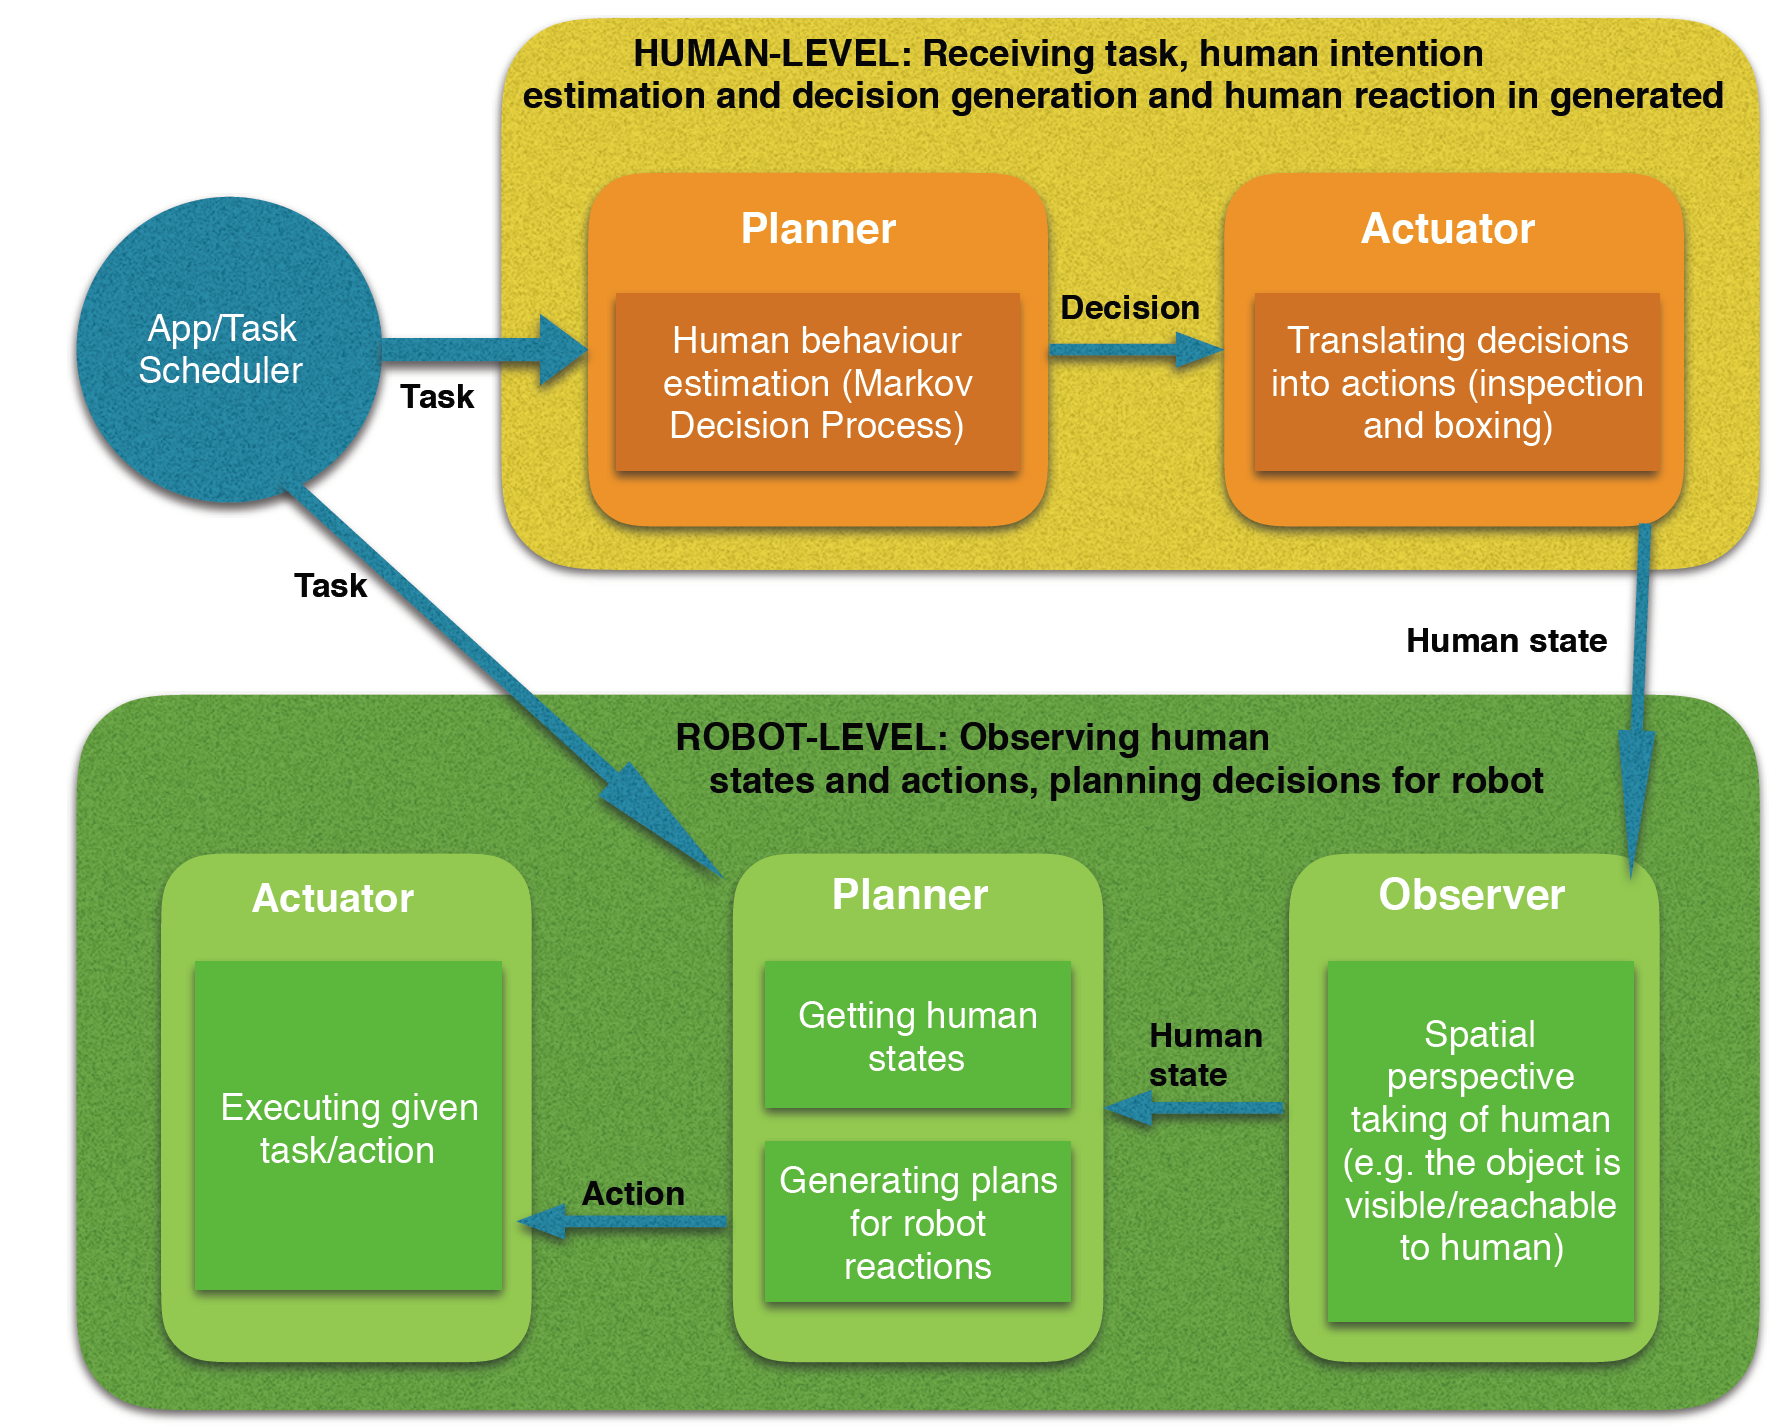
\includegraphics[width=12cm]{Pictures/func/architecture.png}
	\captionof{figure}{general architecture}
	\label{fig:architecture}
\end{minipage}

\begin{minipage}{0.8\textwidth}
\centering
	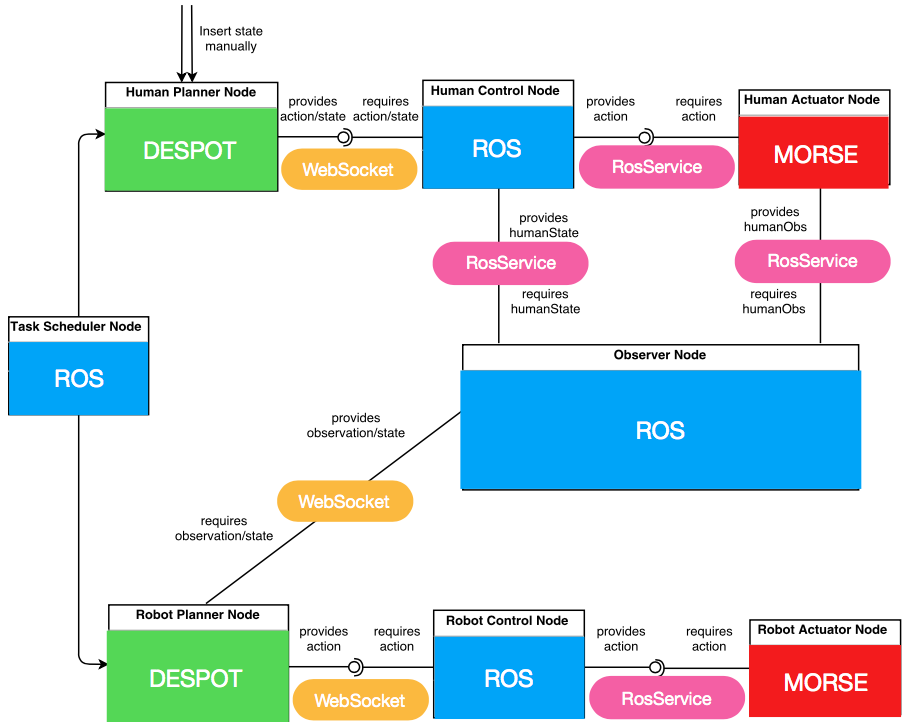
\includegraphics[width=12cm]{Pictures/func/graph.png}
	\captionof{figure}{communication graph}
	\label{fig:graph}
\end{minipage}

\section{Web-Socket and ROS Service}
\subsection{Web-Socket}
This section explains how webSocket works. The reason why we use webSocket is that there are no well-developed ROS packages for MDP or POMDP models. As a substitution, we use the despot library for MDP and POMDP models. To communicate between despot model and ROS, we choose the simple and convenient tool: webSocket.\\
The communication between a client and a serve in webSocket is connected by a identical localhost number. For this project, the localhost numbers used in the three webSocket connections(see Fig \ref{fig:graph}) are 7070, 8080 and 9090. For example, a server with localhost number 7070 is opened and is waiting for a connection. Any client that wants to communicate with this server should declare "connect to server with localhost number 7070". In this way, a client and a server are connected and information can be then transfered between them. (see Fig \ref{fig:webSocket})
 
\subsection{ROS Service}
ROS service is one of the most important communication methods in ROS. There are two nodes in a ROS servive connection: one acts as a client and the other as a server. The connection is specified by an identical and unique ROS service name. A service server has certain pre-defined functions and is always waiting for a request from a service client. If the request is activated, the service server will execute the functions and return a respondse to service client. Fig \ref{fig:ROSservice} shows how ROS service works.

\begin{minipage}{0.4\textwidth}
\centering
	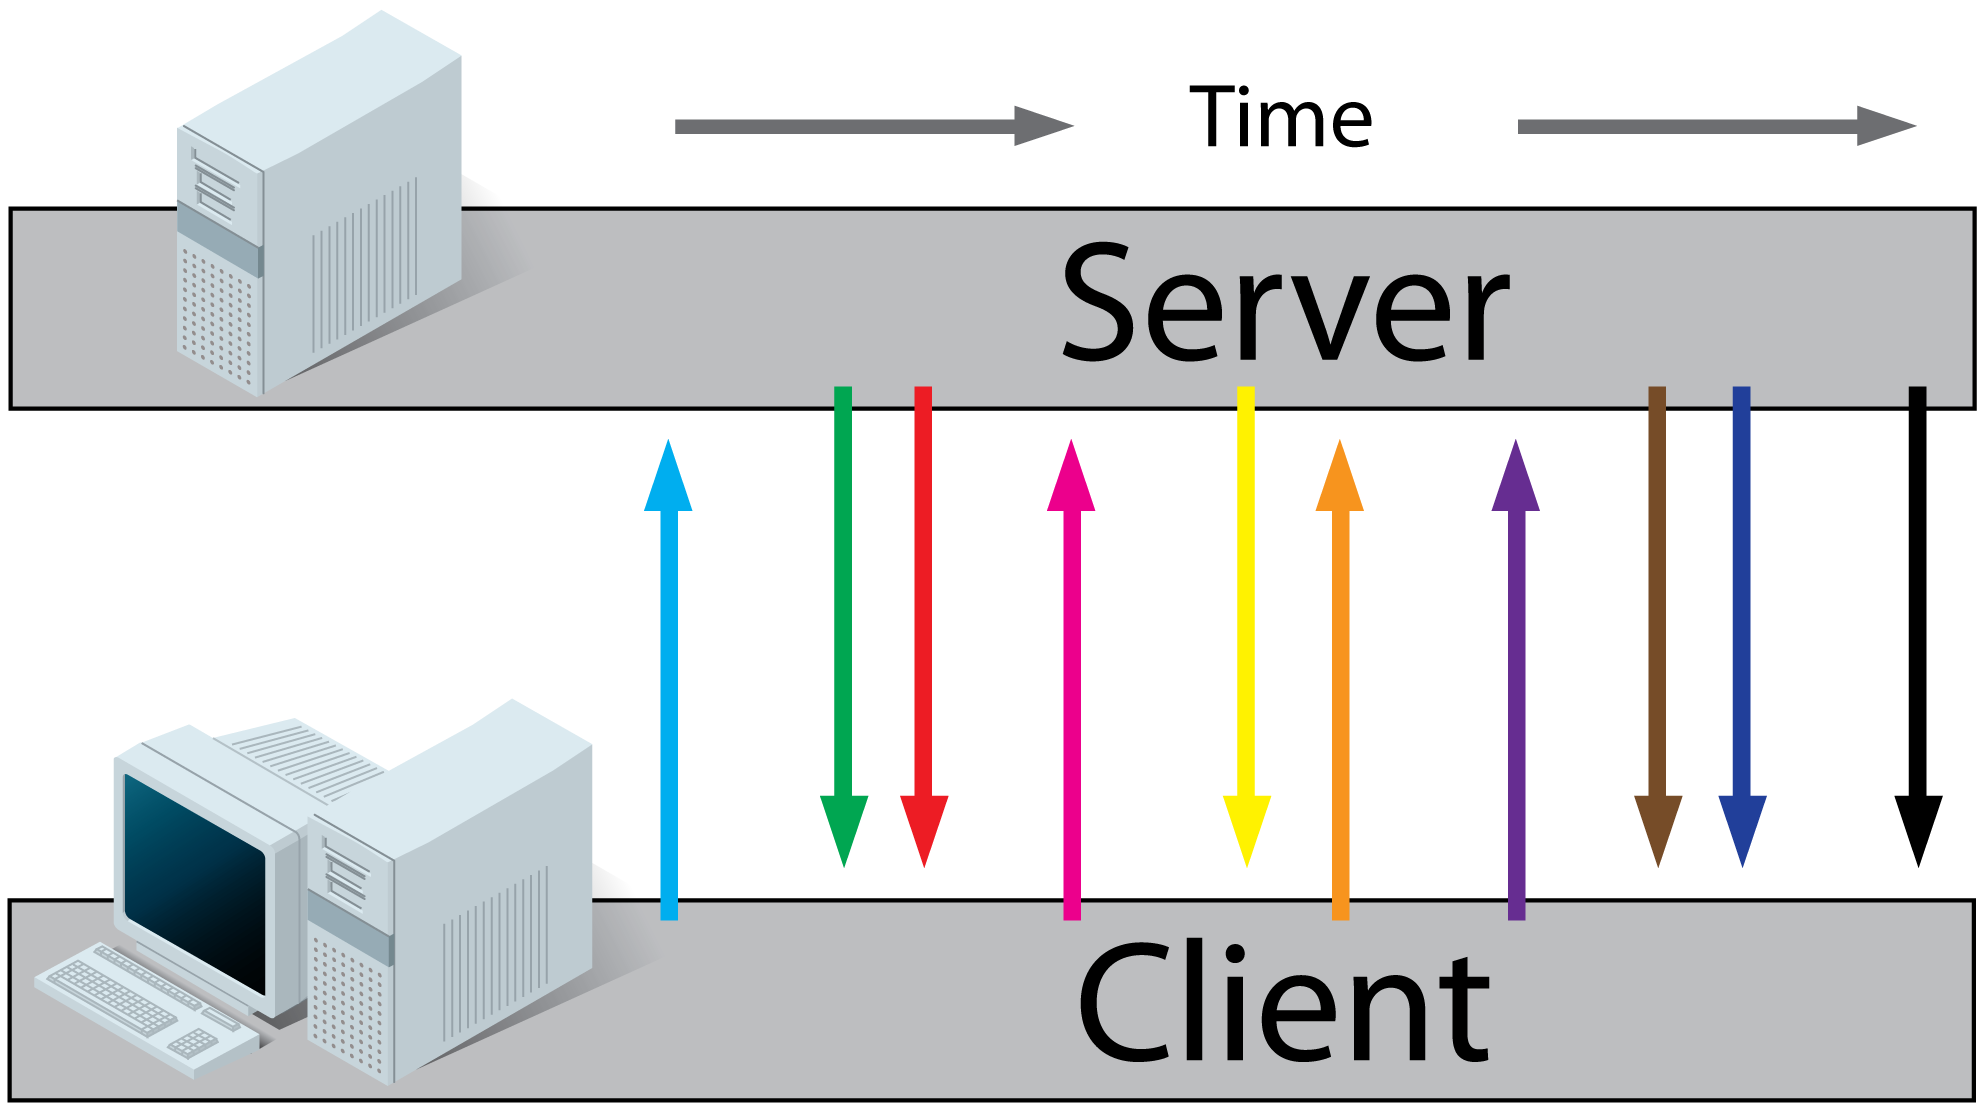
\includegraphics[width=7cm]{Pictures/func/webSocket.png}
	\captionof{figure}{functional theory of webSocket}
	\label{fig:webSocket}
\end{minipage}
\quad\quad\quad\quad
\begin{minipage}{0.4\textwidth}
\centering
	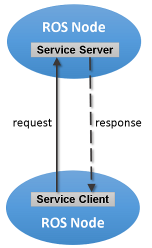
\includegraphics[height=4cm]{Pictures/func/ROSservice.png}
	\captionof{figure}{functional theory of ROS service}
	\label{fig:ROSservice}
\end{minipage}

\section{Morse}
Morse is a generic simulator for academic robotics. It provides a lot of realistic 3D simulations of different environments and autonomous robots. In this project, in order to simulate the collaborate work between a human and robot, we utilize a human component and a P@2 robot component in morse.\\
The current morse platform doesn't feed the need of our project. That's why we need to modify and add some functionalities in the morse source codes. Table \ref{tbl:morsetable} lists a detailed description of all the files that we modify in the project. Table \ref{tbl:ROSservicelist} is a list of all the ROS services that are used in this project.
 
\begin{table}[h]
 	\centering
 	\begin{tabular}{|p{3.5cm}|p{1.5cm}|p{6cm}|}
 		\hline
 		file 				&	change 	&	purpose				\\ \hline
 		human.py			& 	modify		&	1. add the following functionns(declared as ROS service) to simulate the actions of human:	reset; walk away; look around; warn robot; grasp object; attempt to grasp. \\
 							&				& 	2. add the following variables to observe the current states of human: is the object visible to human; is the object reachable to human; if human has the object; what action human is doing.			\\ \hline
 		pr2.py				& 	modify		&	add the following functionns(declared as ROS service) to simulate the actions of robot: reset; open fingers; grasp object; pointto object.																\\ \hline
		human\_overlays.py	&	add			&	This file declares the functions in human.py as ROS services.(See Table \ref{tbl:ROSservicelist} for detailed information of these ROS services.)															\\ \hline
		robot\_overlays.py	&	add			&	This file declares the functions in pr2.py as ROS services.(See Table \ref{tbl:ROSservicelist} for detailed information of these ROS services.)															\\ \hline
		main.py				&	modify		&	The changed codes are in Line 447-467. Our codes make sure that all the components(human, robot, objects) in the scenario can be overlayed as ROS services.											\\ \hline
		human.blend			&	modify		&	reconstruct the components(arm, eyes looking) of human.													\\ \hline
		pr2.blend			&	modify		&	reconstruct the components of robobt																				\\ \hline
		conveyor.blend		&	add			&	a new subject for morse, which simulates the behaviours of a conveyor belt. 										\\ \hline
 	\end{tabular}
 	\caption{Description of all modified files for morse}
 	\label{tbl:morsetable}
\end{table}

\begin{table}[h]
 	\centering
 	\begin{tabular}{|p{4cm}|p{3cm}|p{4cm}|}
 		\hline
 		name of ROS service 	&	name of service type 	&	description			\\ \hline
 		/human/walk\_away		& 	std\_srvs/Trigger		&	execute the action of walking away.						\\ \hline
 		/human/look\_around		& 	std\_srvs/Trigger		&	execute the action of looking around.						\\ \hline
		/human/warn\_robot		&	std\_srvs/Trigger		&	execute the action of raising left arm to warn robot.		\\ \hline
		/human/attempt\_grasp	&	std\_srvs/Trigger		&   execute the action of attemping to grasp the object.		\\ \hline
		/human/grasp			&	std\_srvs/Trigger		&	execute the action of grasping the object.				\\ \hline
		/human/is\_ov			&	std\_srvs/Trigger		&	return if object is visiable to human or not.					\\ \hline
		/human/is\_oir			&	std\_srvs/Trigger		&	return if object is in the range of human or not.		\\ \hline
		/human/is\_ho			&	std\_srvs/Trigger		&	return if human is having the object or not.					\\ \hline
		/human/is\_a0			&	std\_srvs/Trigger		&	return if human is executing the action of attemping to grasp object.		\\ \hline
		/human/is\_a2			&	std\_srvs/Trigger		&	return if human is staying idle and doing nothing.				\\ \hline
		/human/is\_h4			&	std\_srvs/Trigger		&	return if human is executing the action of warning the robot.	\\ \hline
		/human/reset			&	std\_srvs/Trigger		&	put human to initial position. put the object to initial position.				\\ \hline
		/robot/point\_to\_obj	& 	std\_srvs/Trigger		&	execute the action of pointing to the object.				\\ \hline
 		/robot/grasp			& 	std\_srvs/Trigger		&	execute the action of grasping the object.				\\ \hline
		/robot/cancel\_action	&	std\_srvs/Trigger		&	stop current actions and stay idle.							\\ \hline
		/robot/reset			&	std\_srvs/Trigger		&	put robot to initial position.							\\ \hline
 	\end{tabular}
 	\caption{List of all the used ROS services}
 	\label{tbl:ROSservicelist}
\end{table}

\clearpage

\section{MDP}
Finding an implementation solution for designing MDP model was a bit challenging since all implementations sources were documented for POMDP model(Partially Observable MDP) and to overcome this challenge so many search attempts have been made to find an implementation where it can support not only partially observable MDP model but also fully observable MDP model. \\
APPL is a C++ toolkit for approximate POMDP planning which uses XML format to model POMDPx. PomdpX is an XML file format for specifying models of Markov decision processes(MDPs), partially observable Markov decision processes(POMDPs), and mixed observability Markov decision processes(MOMDPs). As a result, the PomdpX file format can specify any of the following models: MDPs, when all state variables are fully observable and POMDPs, when all state variables are partially observable. A PomdpX document consists of a header and a pomdpx root element which in turn contains child elements, Description, Discount, Variable and thereafter: InitialStateBelief, StateTransitionFunction, ObsFunction and RewardFunction. The state, action and observation variables which factorize the state S, action A, and observation O spaces are declared within the Variable element. Reward variables, R are also declared here. By setting fullyobs tag to true, our model will be defined as a fully observable MDP model(see Fig \ref{fig:MDP1}). 

\begin{minipage}{0.8\textwidth}
\centering
	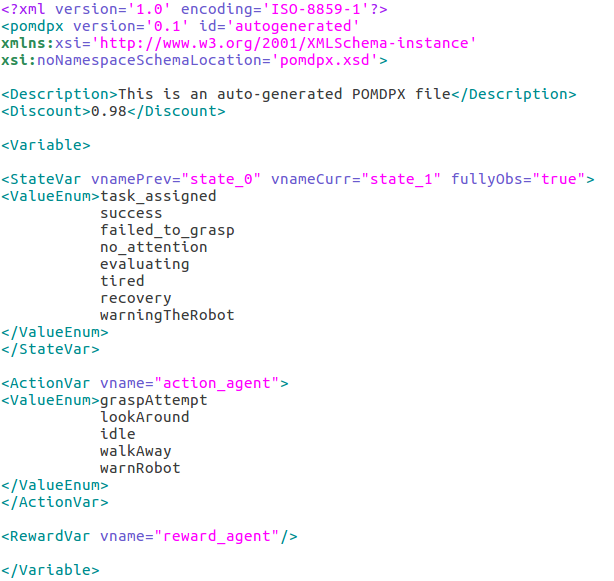
\includegraphics[width=12cm]{Pictures/func/MDP/MDP1.png}
	\captionof{figure}{MDP explanation 1}
	\label{fig:MDP1}
\end{minipage}

We considered S0(task\_assigned) as our initial beliefs state:

\begin{minipage}{0.8\textwidth}
\centering
	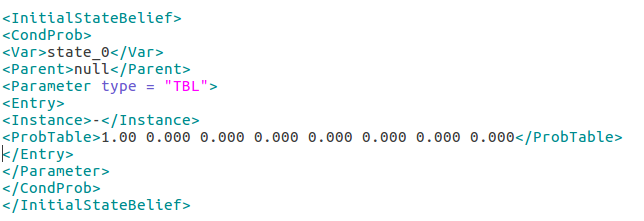
\includegraphics[width=12cm]{Pictures/func/MDP/MDP2.png}
	\captionof{figure}{MDP explanation 2}
	\label{fig:MDP2}
\end{minipage}

Probabilities for each action to reach desired (specified) state:

\begin{minipage}{0.8\textwidth}
\centering
	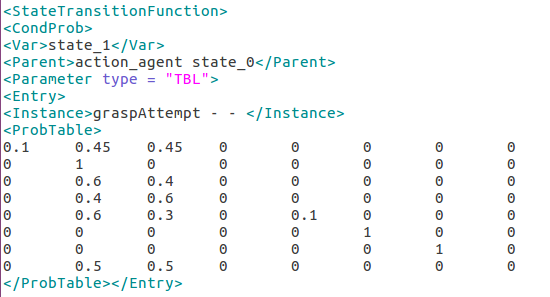
\includegraphics[width=12cm]{Pictures/func/MDP/MDP3.png}
	\captionof{figure}{MDP explanation 3}
	\label{fig:MDP3}
\end{minipage}

And finally rewards for taking actions:

\begin{minipage}{0.8\textwidth}
\centering
	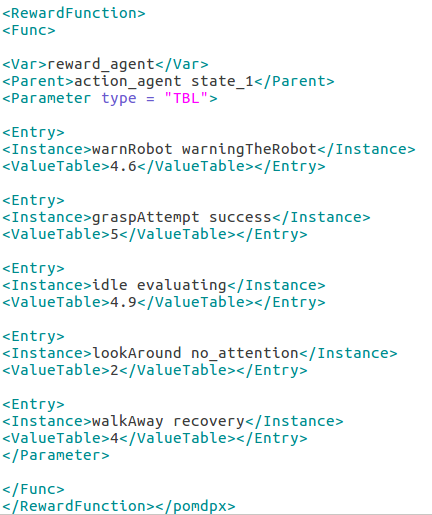
\includegraphics[width=12cm]{Pictures/func/MDP/MDP4.png}
	\captionof{figure}{MDP explanation 4}
	\label{fig:MDP4}
\end{minipage}

To check our model in APPL following commands can be used:

\begin{minipage}{0.8\textwidth}
\centering
	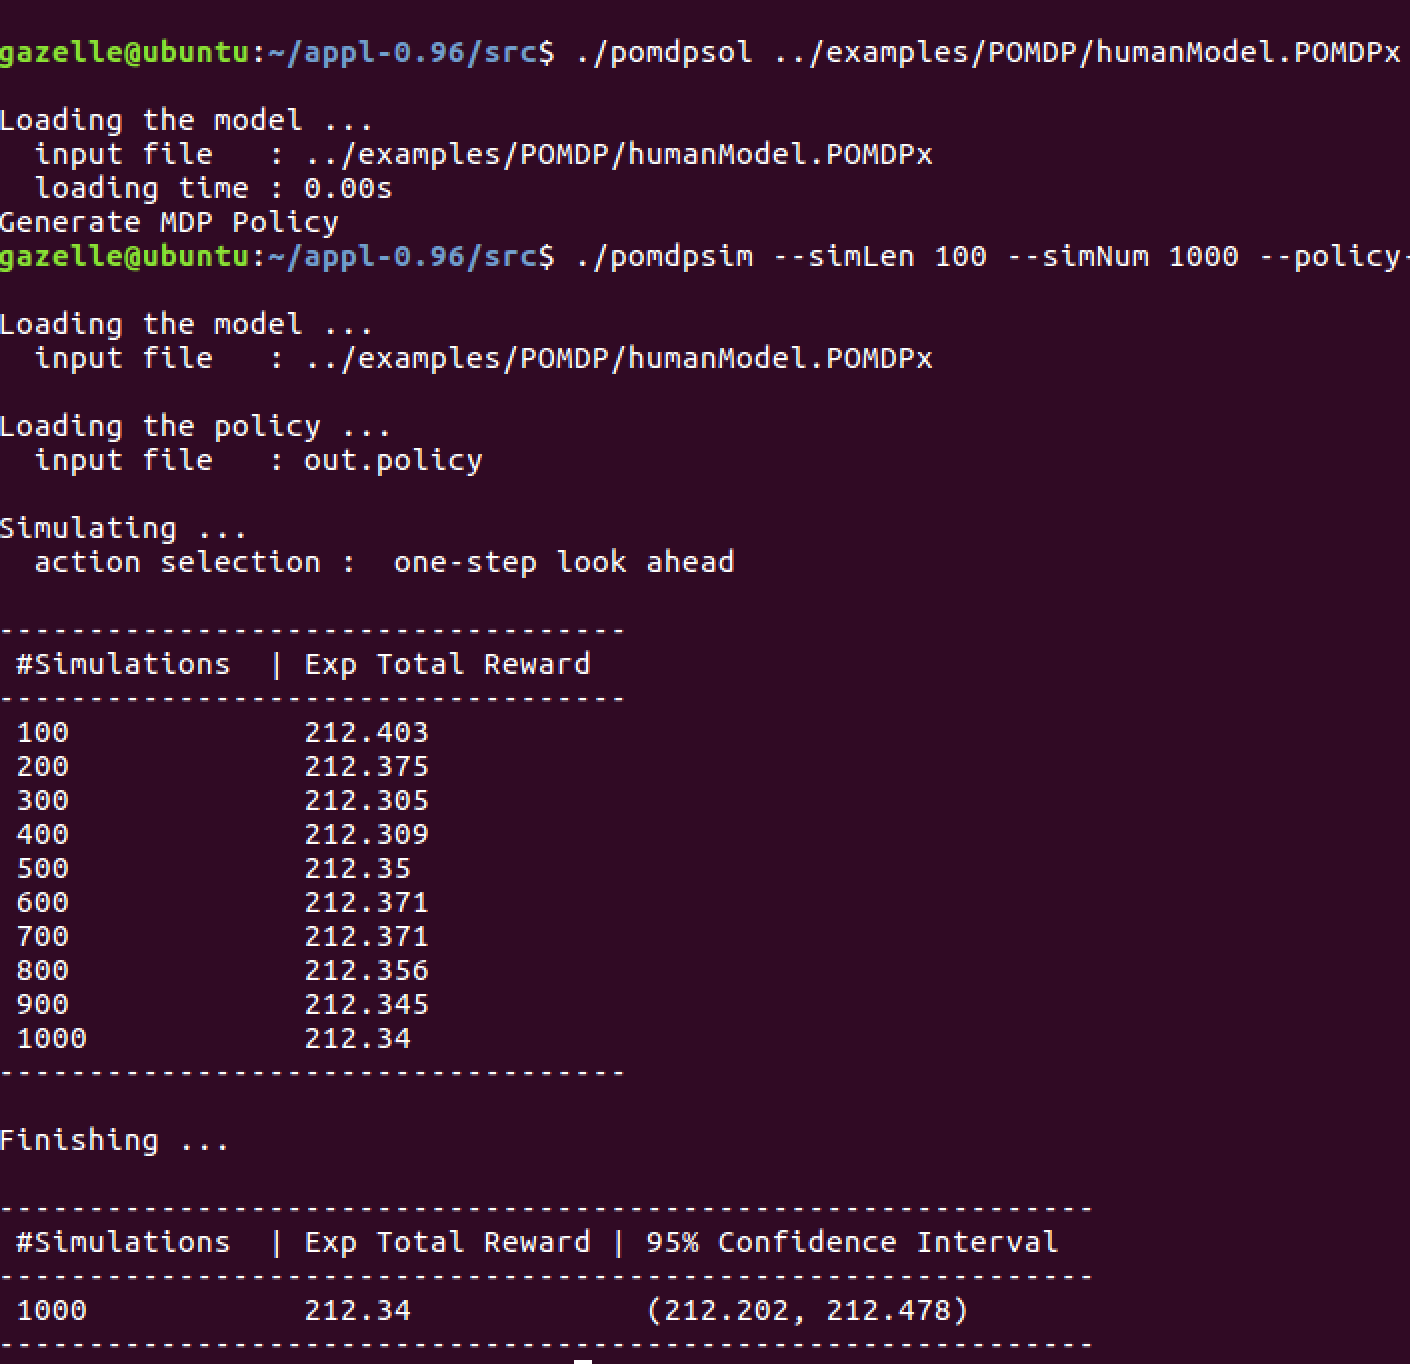
\includegraphics[width=12cm]{Pictures/func/MDP/MDP5.png}
	\captionof{figure}{MDP explanation 5}
	\label{fig:MDP5}
\end{minipage}

As you can see using ./podmpsol command APPL solves provided model and generates policy for that model and to simulate our model ./pomdpsim with number of simulations is provided. In order to run our model and insert states manually, modified version of APPL DESPOT algorithm toolkit have been used. This toolkit is modified by Orhan Can Gorur to insert states manually for our semi-autonomous model. \\
By default DESPOT algorithm follows its own beliefs according to probabilities and reward calculations, therefore no matter what we will input it will follow its own belief estimations. This is good for our fully autonomous model but for semi-autonomous this belief estimations will not allow us to test our few use cases manually and in MDP world removing belief means the sensors values we get(the states in our case) are 100\% true. This gives no randomness, or stochasticity in action selection. Therefore, DESPOT had been adjusted in a way that the state we input comes with noise, and other beliefs are kept too. So, if we enter S4 for the next state, the belief of S4 is always 80\% where the rest of the possible states are added up to 20\%. That gives our human to be skeptical sometimes but still follow the exact states we are inputting in. To change this belief percentage, go to belief.cpp under src/core and edit lines 431 and 434 to adjust this belief distribution.

\begin{minipage}{0.8\textwidth}
\centering
	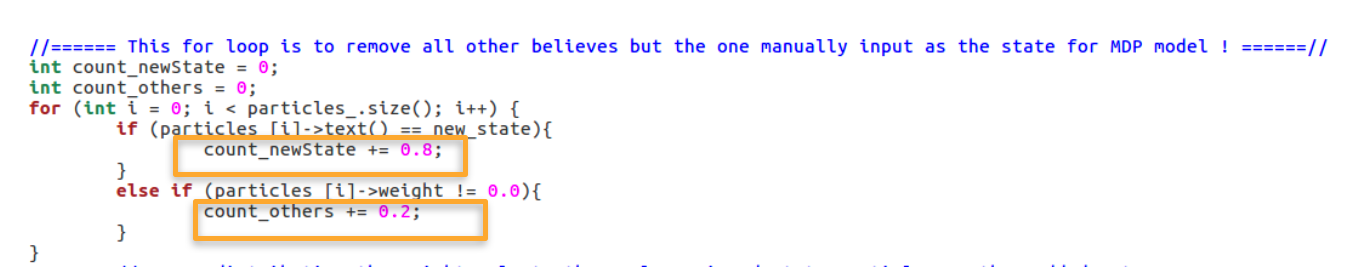
\includegraphics[width=12cm]{Pictures/func/MDP/MDP6.png}
	\captionof{figure}{MDP explanation 6}
	\label{fig:MDP6}
\end{minipage}

We will run Tired Human use case where after many grasp attempts when task is again assigned he will not grasp and will stay idle and after inserting Tired state he will take action walk away and will transit to Recovery state and will not do anything by staying idle.

\begin{minipage}{0.8\textwidth}
\centering
	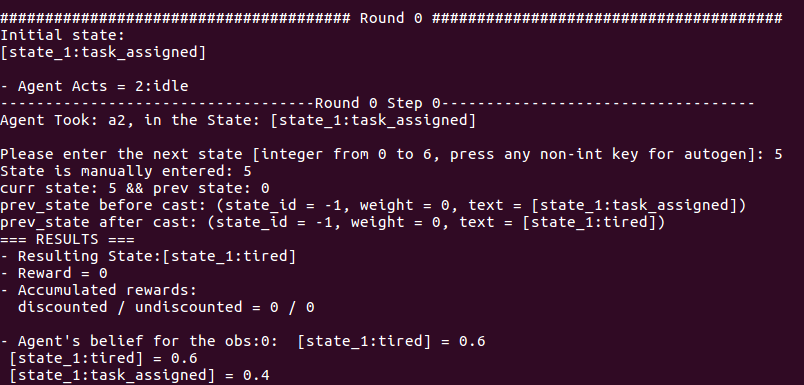
\includegraphics[width=12cm]{Pictures/func/MDP/MDP7.png}
	\captionof{figure}{MDP explanation 7}
	\label{fig:MDP7}
\end{minipage}

\begin{minipage}{0.8\textwidth}
\centering
	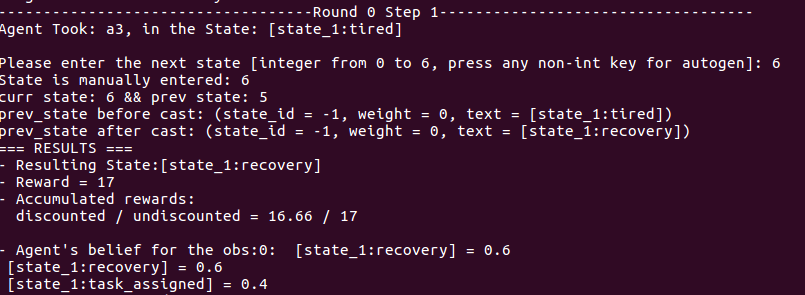
\includegraphics[width=12cm]{Pictures/func/MDP/MDP8.png}
	\captionof{figure}{MDP explanation 8}
	\label{fig:MDP8}
\end{minipage}

\begin{minipage}{0.8\textwidth}
\centering
	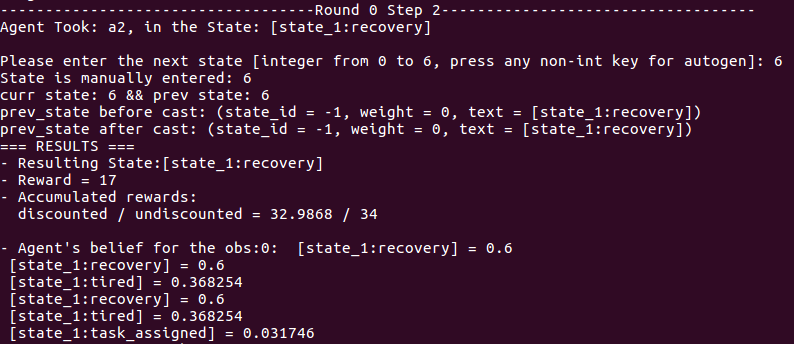
\includegraphics[width=12cm]{Pictures/func/MDP/MDP9.png}
	\captionof{figure}{MDP explanation 9}
	\label{fig:MDP9}
\end{minipage}

Possibilities for following use case are:

\begin{minipage}{0.8\textwidth}
\centering
	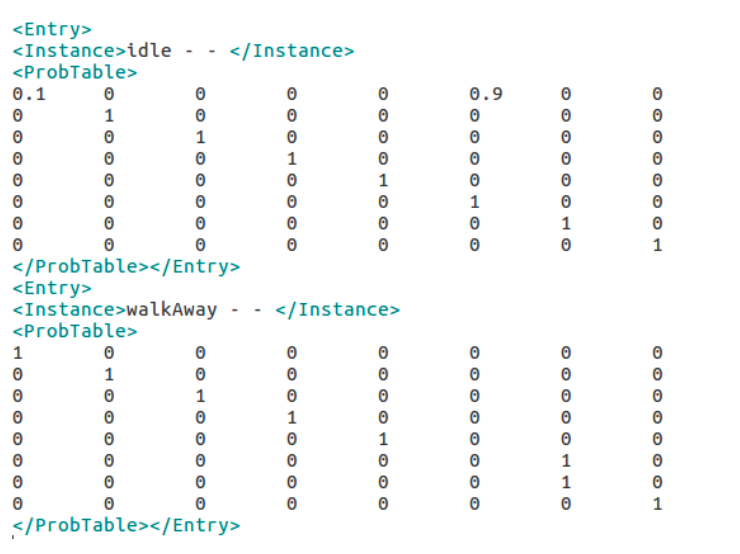
\includegraphics[width=12cm]{Pictures/func/MDP/MDP10.png}
	\captionof{figure}{MDP explanation 10}
	\label{fig:MDP10}
\end{minipage}

And we gave more reward to stay idle in state Recovery and a bit less reward to walk away to reach state Recovery from Tired state. To transit to state Tired from Task Assigned state, we put more probability (90\%) from S0 to S5 to idle action not other actions. \\
For full autonomous model, since we pointed an example of despite inputting manually any state, our agent was following his own beliefs because we set belief to 100\%. Now here we will show a general and bigger picture of fully autonomous model state transitions with random action selections(we considered beginner human).

\begin{minipage}{0.8\textwidth}
\centering
	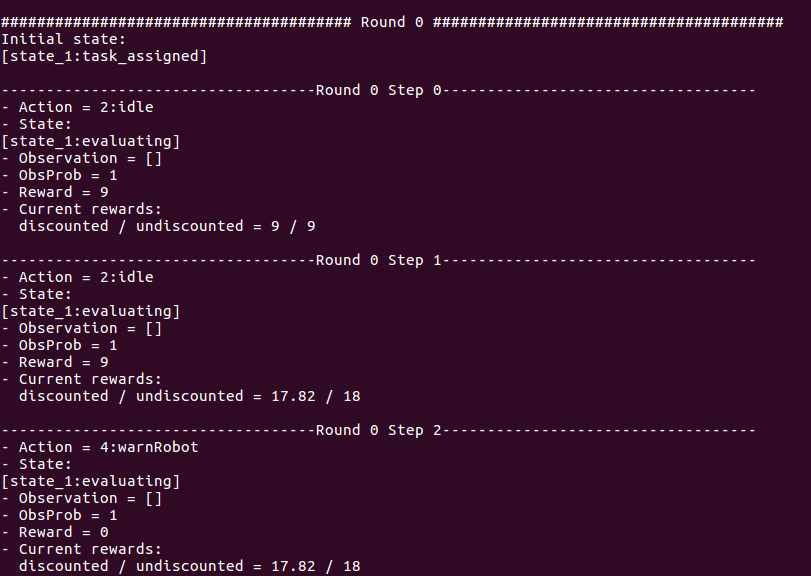
\includegraphics[width=12cm]{Pictures/func/MDP/MDP11.png}
	\captionof{figure}{MDP explanation 11}
	\label{fig:MDP11}
\end{minipage}

\begin{minipage}{0.8\textwidth}
\centering
	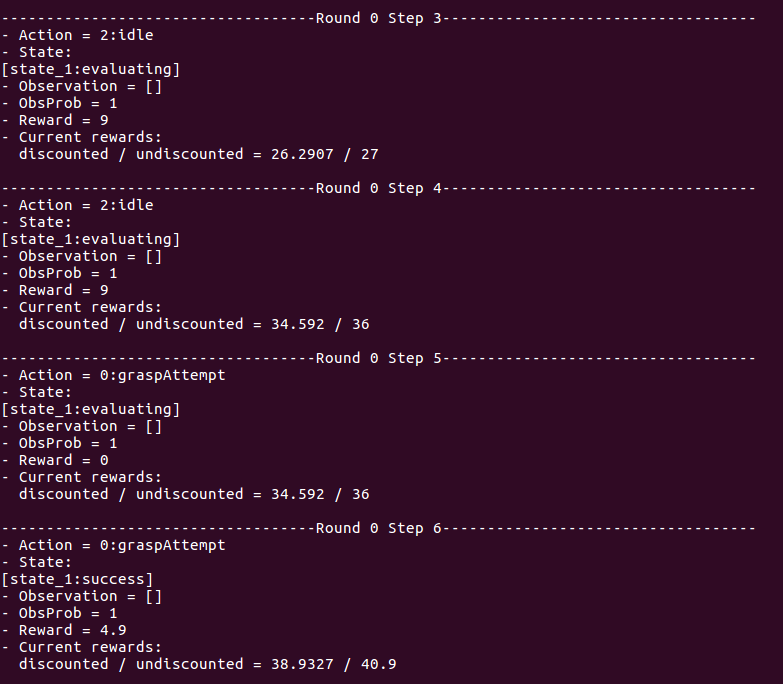
\includegraphics[width=12cm]{Pictures/func/MDP/MDP12.png}
	\captionof{figure}{MDP explanation 12}
	\label{fig:MDP12}
\end{minipage}

\clearpage

\section{POMDP}

POMDP will help the robot to estimate the current state human might be in and based on that take an action to help reach human its desired state (SUCCESS state). The pomdp file consists of 8 parts, which include: 1.The Discount value and definition of rewarding; 2.The human state belief (estimation by robot); 3.Robot actions; 4.Observations based on the environment; 5.Initial Belief probability (starting state); 6.State Transitions for robot action; 7.Observation Probabilities for estimated state of human and 8.Rewards for taken actions.

\begin{minipage}{0.8\textwidth}
\centering
	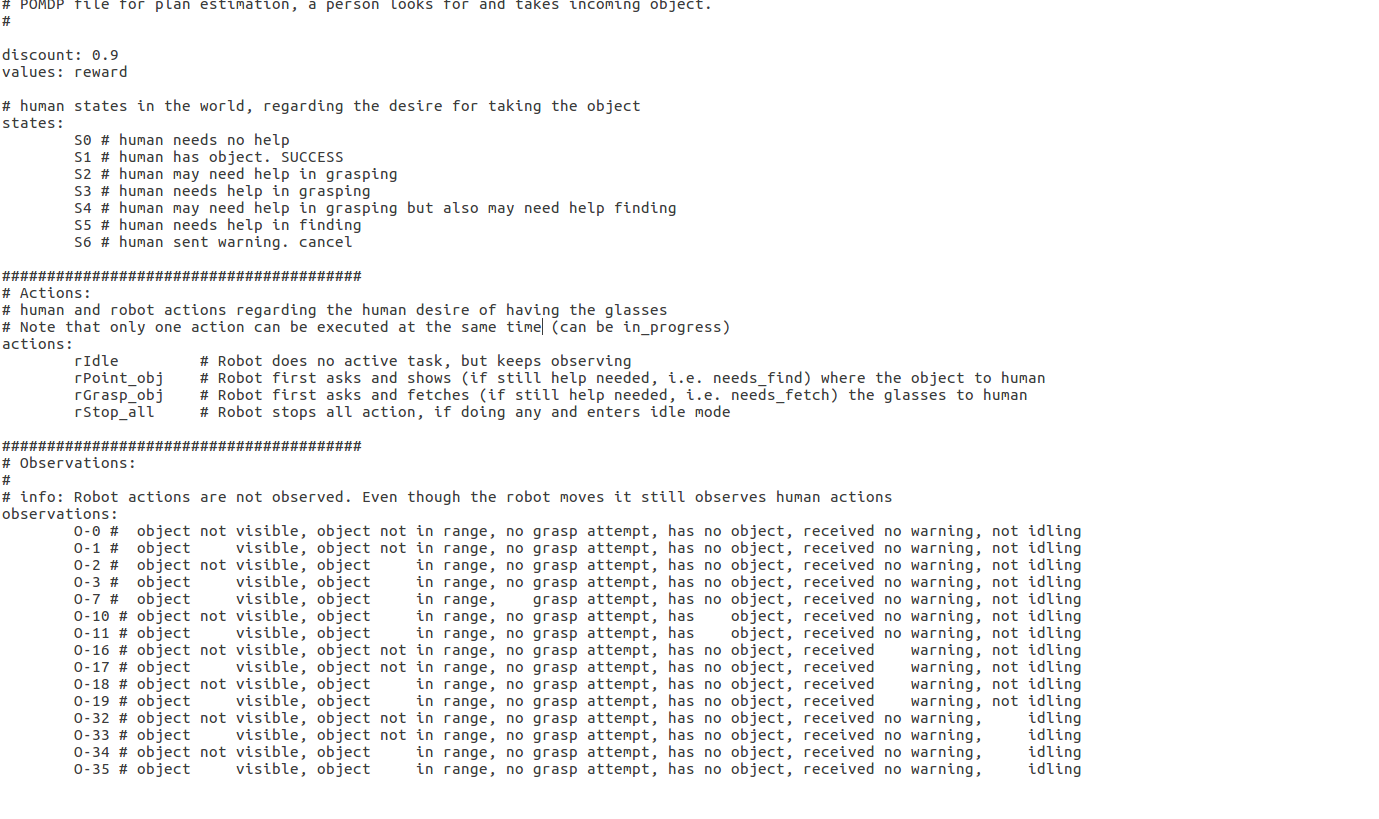
\includegraphics[width=12cm]{Pictures/func/POMDP/POMDP1.png}
	\captionof{figure}{Discount, Human State Beliefs, Robot action and Observations}
	\label{fig:POMDP1}
\end{minipage}

In Figure \ref{fig:POMDP1} you can see the estimated human belief states for robot. A discount value near “1” means, that every action taken and thus the given reward is accounted immediately, which means that the robot gets encouraged in a short term through positive rewarding. A low value for “discount” would make the robot think in a “long-term” process which means that robot might take negative action in an approach to achieve good results at the end.\\
Figure \ref{fig:POMDP2} describes with which probability robot will transition from state x to state y. For example for the first matrix (robot action: idle), first row, robot has the probability of 30\% to stay in its initial state (state 0), has 40\% chance to go from state 0 to state 1 and 15\% each to go from state 0 to either state 2 or 4.

\begin{minipage}{0.8\textwidth}
\centering
	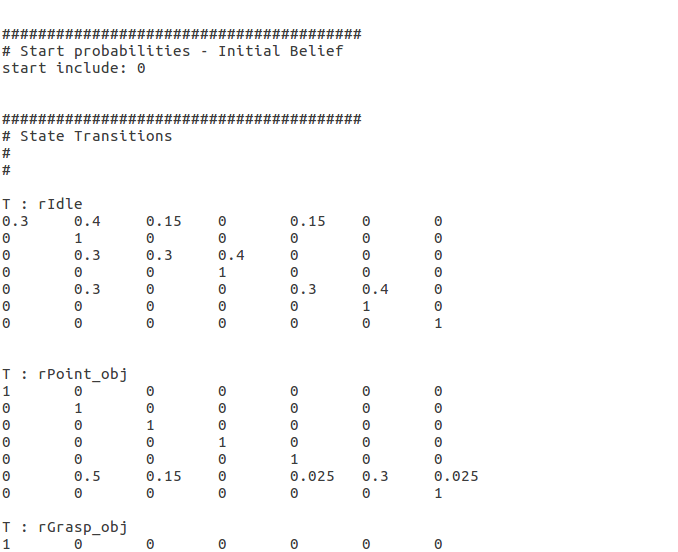
\includegraphics[width=12cm]{Pictures/func/POMDP/POMDP2.png}
	\captionof{figure}{Start probabilities and State transitions}
	\label{fig:POMDP2}
\end{minipage}

In Figure \ref{fig:POMDP3} you see the probabilities that can be emitted from each state, based on the state and action robot is in. The columns are different observations (see figure 1 for further explanation) and the states are rows.

\begin{minipage}{0.8\textwidth}
\centering
	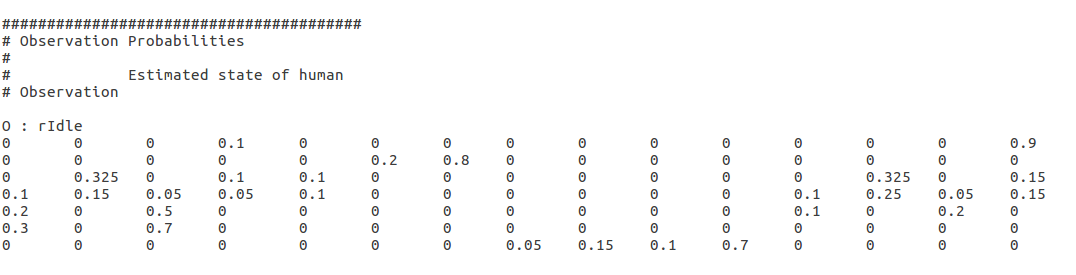
\includegraphics[width=12cm]{Pictures/func/POMDP/POMDP3.png}
	\captionof{figure}{Observations}
	\label{fig:POMDP3}
\end{minipage}

Figure \ref{fig:POMDP4} shows the reward table for certain actions. In this Scenario we want the robot to be heavily encouraged of taking the object and successfully enter state 1 after that (SUCCESS state), while punishing actions we do not desire in certain states. This might be idling in unsuitable situations (here: states), for instance when the human needs help in grasping or finding the object ( = idling in state s3, s5, s6 will lead into punish). Also slightly punish the robot for doing wrong actions like pointing when the robot should be grasping and vice versa.

\begin{minipage}{0.8\textwidth}
\centering
	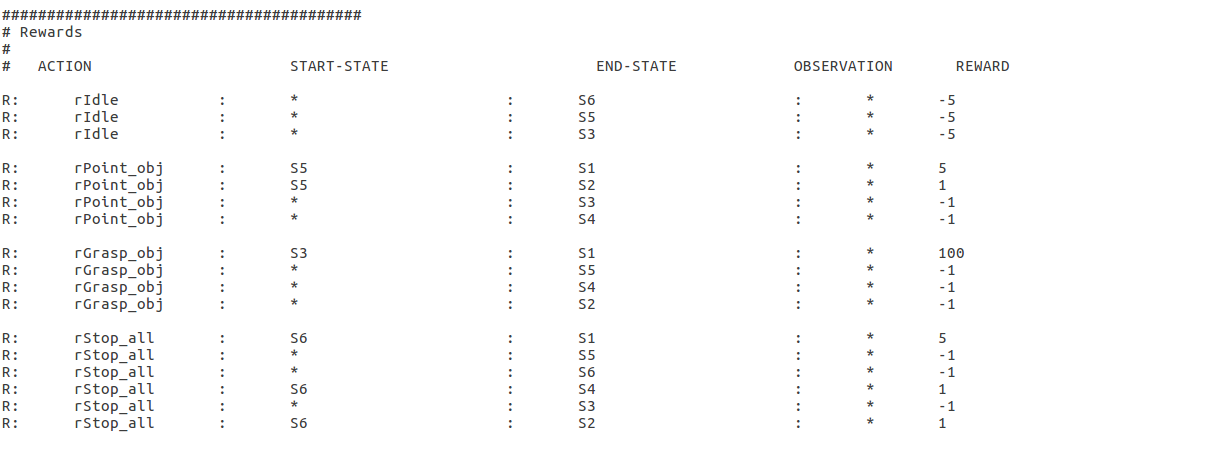
\includegraphics[width=12cm]{Pictures/func/POMDP/POMDP4.png}
	\captionof{figure}{Rewards for actions}
	\label{fig:POMDP4}
\end{minipage}
